 
\documentclass[10pt]{article}         %% What type of document you're writing.
\usepackage{graphicx}
\usepackage{hyperref}
\usepackage[dvipsnames]{xcolor}

%%%%% Preamble

%% Packages to use

\usepackage{amsmath,amsfonts,amssymb}   %% AMS mathematics macros

%% Title Information.

\title{Red Neuronal (Alfabeto griego)}
\author{Denisse Arely Gonzalez Santos}
%% \date{2 July 2004}           %% By default, LaTeX uses the current date

%%%%% The Document

\begin{document}

\maketitle

\begin{abstract}
This document implements the neural network for Greek alphabet.
\end{abstract}

\section{Introduccion}

El presente trabajo es un reporte tecnico del desarrollo de una red neuronal,antes de empezar definiremos que es una red neuronal.
\\Las redes neuronales artificiales (también conocidas como sistemas conexionistas) son un modelo computacional el que fue evolucionando a partir de diversas aportaciones científicas que están registradas en la historia Consiste en un conjunto de unidades, llamadas neuronas artificiales, conectadas entre sí para transmitirse señales. La información de entrada atraviesa la red neuronal (donde se somete a diversas operaciones) produciendo unos valores de salida.

Ademas de comprender el proceso de toma de decisiones y cómo las tecnologías de información, en
especial la inteligencia artificial con el manejo de redes neuronales, pueden servir de apoyo
a dicho proceso, es el objetivo central de este trabajo de investigación, el cual se ha
actualizado y ha permitido revisar los resultados de la red neuronal.

\begin{figure}[htb]
\centering
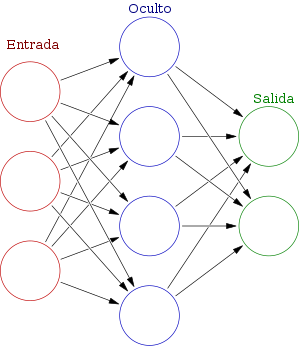
\includegraphics[width=0.2\textwidth]{red neuronal.png}
\caption{Red neuronal}
\label{fig:tigre}
\end{figure}


\section{Desarrollo}
A continuacion hablare sobre mi red neuronal primero mi tema sera sobre el alfabeto griego que consta de 24 letras.
De aqui en adelante hacemos el prototipo en Octave que reemplaza a matlab, crearemos matrices de tamaño 13x13, para saber cuantas figuras podran ser reconocidas por la red neuronal ocuparemos la siguiente formula primero encontraremos N que es el resultado de la multiplicacion del tamaño de la matriz 13*13, despues de obtener N (numero de datos), 169*0.15=25.25 que este resultado seria el total de figuras que seran reconocidas. Despues de realizar el maquetado en octave creamos la red neuronal en el lenguaje de programacion c++.

Para entrenar la red neuronal se debe usar Octave que está desarrollado en MATLAB Para lograrlo, en nuestro caso, hemos seguido los siguientes pasos:
Representar los patrones de la matriz: para representar tanto los símbolos del teclado se usó una matriz de 13*13, para representar un símbolo en dicha matriz, será poner el valor uno (1) en las celdas por donde pasa la marca del número y el valor menos uno (-1) en caso contrario.

Despues de que se comprobo que funcionara como lo esperado se empezara a crear el codigo de la red neuronal en c++, en este caso la matriz se representara sera poner el valor 1 en las celdas por donde pasa el marca del numero y el valor 0 en caso contrario rellenando una matriz de 13 * 13 como se puede observar en la figura 2.

\begin{figure}[htb]
\centering
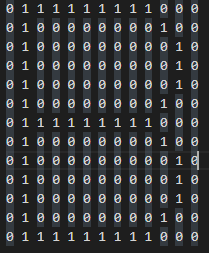
\includegraphics[width=0.3\textwidth]{entrada.png}
\caption{Patron de entrada}
\label{fig:tigre}
\end{figure}

En nuestro caso el patron de entrada si fue reconocido, se muestra la salida en la siguiente figura 3.

\begin{figure}[htb]
\centering
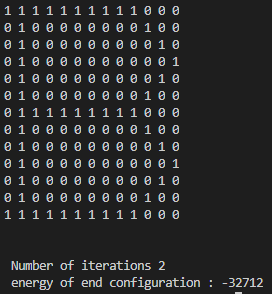
\includegraphics[width=0.2\textwidth]{salida.png}
\caption{Patron de salida}
\label{fig:tigre}
\end{figure}

Por lo tanto, como en nuestro caso solamente deseamos reconocer, en nuestro caso el patron de entrada si fue reconocido.

\section{Conclusion}
 Como resultado de este trabajo podemos concluir que el uso de las Redes Neuronales es una gran alternativa para la solucion de muchos probelmas.

Usando como base los resultados mostrados podemos resolver prblemas mas complejos, realidad que representa este trabajo es que es una solucion muy basica, pero al mismo tiempo creo que permite apreciar en detalle la entrada y salida sobre el reconocimiento de patrones que es la base de la vision artificial.

\end{document}